%!TEX TS-program = xelatex
%!TEX encoding = UTF-8 Unicode
%!BIB TS-program = biber
\documentclass[letterpaper,11pt]{article}

\usepackage{fontspec,silence,csquotes,booktabs,multirow,filecontents}

\usepackage{tikz}
\usepackage{tikz-qtree}

\setmainfont{Linux Libertine}

\usepackage[margin=1in]{geometry}

% Prevent (sub)section titles appearing by themselves at end of page
\usepackage{titlesec}

\titlespacing*{\section}{0pt}{0.65\baselineskip}{0.5\baselineskip}
\titlespacing*{\subsection}{0pt}{0.65\baselineskip}{0.5\baselineskip}
\titleformat*{\section}{\fontspec{Alegreya Sans SC}}
\titleformat*{\subsection}{\normalsize\itshape}
\titleformat*{\subsubsection}{\normalsize\bfseries}

\usepackage[british]{babel}
\usepackage[backend=biber,natbib=true,style=apa,url=true]{biblatex}
\DeclareLanguageMapping{british}{british-apa}
\addbibresource{report.bib}

\WarningFilter{biblatex}{Patching footnotes failed}

\usepackage[colorlinks=true,linkcolor=blue,citecolor=blue,filecolor=blue,urlcolor=blue]{hyperref}

\usepackage[labelfont=bf]{caption}

\newcommand\blfootnote[1]{%
  \begingroup
  \renewcommand\thefootnote{}\footnote{#1}%
  \addtocounter{footnote}{-1}%
  \endgroup
}

\definecolor{cbred}{HTML}{e41a1c}
\definecolor{cbblu}{HTML}{377eb8}
\definecolor{cbpur}{HTML}{984ea3}
\definecolor{cbgrn}{HTML}{4daf4a}
\definecolor{cborn}{HTML}{ff7f00}

\begin{document}

\noindent{}{\fontspec{Alegreya Sans SC}Report}

\begin{center}
\vspace{2em}
\noindent {\LARGE Rapid generalization in phonotactic learning: a replication project}
\vspace{2em}

\noindent {\large Nay San*\blfootnote{*Many thanks to Judith Degen for providing the opportunity and resources to make this class project possible, as well as Tal Linzen and Gillian Gallagher for having made their experiment materials readily available on GitHub along with helpful correspondance during the construction of my replication experiment. Any errors introduced are my own.}}
\vspace{2em}

\noindent {June 2020}
\end{center}

\section{Introduction}

Natural languages place various restrictions on how sounds may combine to create words, and phonotactics is the set of these restrictions.
For example, in English phonotactics, while the velar nasal sound [ŋ] is permissble word-finally, e.g. \emph{king} [kɪŋ], it is not permissble word-initially, e.g. *[ŋɪk] (even though other nasals are, e.g. \emph{nick} [nɪk]).
By contrast, in many other languages word-initial [ŋ] is entirely permissble: e.g. [ŋo] meaning \emph{to cry} in Burmese.
Language learners are virtually never given explicit instruction about these restrictions, yet they come to have intuitions about how words in the target language should sound.
In essence, language learners automatically form generalisations about the phonotactics of a language based on their exposure to words in the language.
How varying amounts of exposure to an artificial language effects phonotactic generalisations about the language was investigated by \textcite{linzen2017rapid} in a series of four experiments.
In this report, I present results from a replication experiment based on one of these experiments.

\section{Background: Linzen \& Gallagher (2017)}

Sensitivity to phonotactically legal and illegal sequences of sounds has been shown across a variety of experiments, including artificial language learning experiments.
In these experiments, participants are exposed to a set of words from a miniature artificial language in an exposure (or training) stage and in a subsequent testing stage complete a series of judgement tasks to establish what knowledge about the language they have inferred from the exposure stage.
Previous studies investigating phonotactic learning, however, typically provide participants with a large amount of exposure to the artificial language.
Thus, little is known about the early stages and the time course of phonotactic learning, prompting the questions: How much exposure to the language is needed before learners form generalisations? Are multiple instances of a certain phonological feature required to prompt generalisations? How does the likelihood of generalisation change with more instances?

To gather empirical data towards addressing these questions, \textcite{linzen2017rapid} conducted 4 experiments investigating phonotactic learning.
In brief, each subsequent experiment altered the basis on which generalisations may be formed: in Experiment 1, the participants were presented with categorical data (all consonants of interest in the exposure stage shared the relevant phonological feature).
In Experiments 2a and 2b, they were probabilistic: a fraction of the data were phonotactically legal. 
Finally, whether or how participants generalised from a single instance of a sound was investigated in Experiment 3.
Given the increased complexity in the composition of artificial languages in each subsequent experiment, more participants were needed in the later experiments (e.g. 450 in Experiment 3 vs. 288 in Experiment 1).
Given the constraints of a class project, I chose to replicate Experiment 1, and thus only focus on details of Experiment 1 in the remainder of this section.

\newpage

\subsection{Materials}

Table \ref{tab:stim} provides an overview of the stimuli used by \textcite{linzen2017rapid}.
To create the artificial languages for the experiment, 540 nonce-words of the form C\textsubscript{1}V\textsubscript{1}C\textsubscript{2}V\textsubscript{2}(C\textsubscript{3}) were recorded by a native English speaker.
The word-initial consonants (the segments of interest) were drawn from a set of six voiced obstruents [b d g v z ð] and six voiceless obstruents [p t k f s θ], whose phonological features are provided in Table (1b).

Table (1c) provides an overview of the counter-balancing design, in which each row of 3 consonants provide the basis of an artificial language, which consists only of voiced consonants (Lists 1-6) or voiceless consonants (Lists 7-12) --- n.b. the non-conforming consonant in the third column has the opposite voicing of those in the previous 2 columns (as indiciated by the blue vs. red text colour).
Note that while the conforming consonants share voicing, the non-conforming consonant shares the same place of articulation as the unattested but conforming one, e.g. [b] and [p] in List 1 are both labial consonants (as indicated by the underlining).

\begin{table}[h]
\centering
\caption{Stimulus design from \textcite{linzen2017rapid}. Table (a) describes the composition of the 540 stimulus items. Table (b) lists the phonological features of the consonants of interest, C\textsubscript{1}. Table (c) reports the counter-balancing design.}
\label{tab:stim}
(a)
\begin{tabular}{ccc}
{\renewcommand\arraystretch{1.5}\begin{tabular}{@{}ccccc@{}}
\\\toprule
C\textsubscript{1} & V\textsubscript{1} & C\textsubscript{2} & V\textsubscript{2} & (C\textsubscript{3}) \\ \midrule
b  & a  & l  & a  & -    \\
ð  & e  & m  & i  & -    \\
d  & i  & n  & u  & -    \\
f  & o  & l  & i  & -    \\
t  & u  & n  & a  & l    \\
\bottomrule
\end{tabular}} & where &
{\begin{tabular}{l}
C\textsubscript{1} $\in$ \{ p, t, k, f, θ, s, b, d, g, v, ð, z \} \\
V\textsubscript{1} $\in$ \{ a, e, i, o, u \} \\
C\textsubscript{2} $\in$ \{ l, m, n \} \\
V\textsubscript{2} $\in$ \{ a, i, u \} \\
C\textsubscript{3} $\in$ \{ l, m, n \}, if C\textsubscript{1}V\textsubscript{1}C\textsubscript{2}V\textsubscript{2} is an English word (e.g. \emph{tuna}) \\
\\
Total stimulus items = 540 = 12 $\times$ 5 $\times$ 3 $\times$ 3\\
\hphantom{Total stimulus items = 540} = |C\textsubscript{1}| $\times$ |V\textsubscript{1}| $\times$ |C\textsubscript{2}| $\times$ |V\textsubscript{2}| \\
    \hphantom{f}
\end{tabular}}
\end{tabular}

\begin{tabular}{@{}cccccc@{}}
\multicolumn{6}{c}{(b)} \\
\toprule
\multirow{2}{*}[-1em]{Voicing} & \multirow{2}{*}[-1em]{Manner} & \multicolumn{4}{c}{Place of articulation}                                                      \\ \cmidrule(l){3-6} 
                         &                         & Labial & \multicolumn{2}{c}{Coronal} & Dorsal \\ \midrule
{\color{cbred}Voiceless}                & Stop                 & \underline{p}                                                             &             & \textbf{t}        & \emph{k}     \\  \cmidrule(l){3-6}
{\color{cbred}Voiceless}                & Fricative               & \underline{f}                                                             & \textbf{θ}           & \textbf{s}        &       \\ \cmidrule(l){2-6} 
{\color{cbblu}Voiced}                & Stop                 & \underline{b}                                                             &             & \textbf{d}        & \emph{g}     \\   \cmidrule(l){3-6}
{\color{cbblu}Voiced}                & Fricative               & \underline{v}                                                             & \textbf{ð}           & \textbf{z}        &       \\ \bottomrule
\end{tabular}
\begin{tabular}{@{}c|c|cc@{}}
\multicolumn{4}{c}{(c)} \\
\toprule
& & \multicolumn{2}{c}{Unattested} \\
\multirow{2}{*}[1.25em]{List ID} & \multirow{2}{*}[1.25em]{Attested}                     &  Conforming                       & Non-conforming                      \\ \midrule
1       & {\color{cbblu}\emph{g}} & {\color{cbblu}\underline{b}} & {\color{cbred}\underline{p}}  \\
2       & {\color{cbblu}\textbf{z}} & {\color{cbblu}\textbf{d}} & {\color{cbred}\textbf{t}}\\
3       & {\color{cbblu}\textbf{ð}} & {\color{cbblu}\emph{g}} & {\color{cbred}\emph{k}} \\
4       & {\color{cbblu}\textbf{d}} & {\color{cbblu}\underline{v}} & {\color{cbred}\underline{f}}                              \\
5       & {\color{cbblu}\underline{v}} & {\color{cbblu}\textbf{z}}                            & {\color{cbred}\textbf{s}}                             \\
6       & {\color{cbblu}\underline{b}} & {\color{cbblu}\textbf{ð}}                            & {\color{cbred}\textbf{θ}}                             \\
7       & {\color{cbred}\emph{k}}                           & {\color{cbred}\underline{p}}                            & {\color{cbblu}\underline{b}}  \\
8       & {\color{cbred}\textbf{s}}                           & {\color{cbred}\textbf{t}}                            & {\color{cbblu}\textbf{d}} \\
9       & {\color{cbred}\textbf{θ}}                           & {\color{cbred}\emph{k}}                            & {\color{cbblu}\emph{g}}                             \\
10      & {\color{cbred}\textbf{t}}                           & {\color{cbred}\underline{f}}                            & {\color{cbblu}\underline{v}}                             \\
11      & {\color{cbred}\underline{f}}                           & {\color{cbred}\textbf{s}}                            & {\color{cbblu}\textbf{z}}                             \\
12      & {\color{cbred}\underline{p}}                           & {\color{cbred}\textbf{θ}}                            & {\color{cbblu}\textbf{ð}}                             \\
\bottomrule
\end{tabular}
\end{table}

\subsection{Procedure}

At the start of each experiment, participants were assigned to a specific list (e.g. List 11) and a specific number of exposures (e.g. 1-set).
With these two parameters, stimuli that were compatible with the list were drawn randomly from the pool of 540 items at run time.
For example, given that List 11 is a voiceless language where [s] is to be the held out consonant, the remaining 5 voiceless obstruents are [p t k f θ].
Thus, in a 1-set condition, 5 words beginning with these consonants (e.g. [pinu], [tanu], [kelo], [fula], [θomi]) would be randomly drawn for the exposure stage of the experiment.
For the 2-, 4-, and 8-set conditions, multiple sets were drawn such that the frequency of occurence of each word-initial consonant remained the same at 20\% (e.g. in the 2-set condition with a total of 10 words, there would be exactly two [p/t/k/f/θ]-initial words).
Thus the exposure stage may vary from 5 trials (1-set) to 40 trials (8-set).

Regardless of the length of exposure, the testing stage consisted of 6 trials for all participants.
For the testing stage, two additional words that begin with the attested consonant were drawn, e.g. [falu] and [femi] for [f] (i.e. not [fula] heard in the exposure stage), along with two that begin with the held-out consonant, e.g. [soma] and [sunu] for [s], and the non-conforming consonant, e.g. [zila] and [zoma] for [z].
In each trial in the testing stage, participants were asked ``Does this sound like it could be a word of the language you were listening to?''.
The presentation order of the stimuli were randomised within both the exposure and testing stages of the experiment.

\subsection{Participants}

For each of the exposure conditions (1-, 2-, 4-, or 8-set), 72 participants were recruited on Amazon Mechanical Turk (MTurk) --- six participants for each each of the 12 lists in Table 1c ---, yielding a total of 288 participants ($288 = 4 \times 6 \times 12$).
Three participants were rejected as their reported native language was not English. Thus \textcite{linzen2017rapid} reported results based on responses from 285 participants.

\subsection{Results}

Figure \ref{fig:lng} displays the mean endorsement rates for each exposure condition (1-, 2-, 4-, 8-sets) and stimulus type (conforming-attested, conforming-unattested, or nonconforming-unattested) reported by \textcite{linzen2017rapid}.
The two key results are that 1) there was no main effect of exposure on endorsement rate and that 2), within each exposure group, the nonconforming-unattested stimuli (blue squares in Figure 1) were endorsed significantly less than conforming-attested stimuli (red circles in Figure 1).
Additional results from \textcite{linzen2017rapid} will be discussed below in comparison the results of the replication experiment.

\begin{figure}[h]
\center
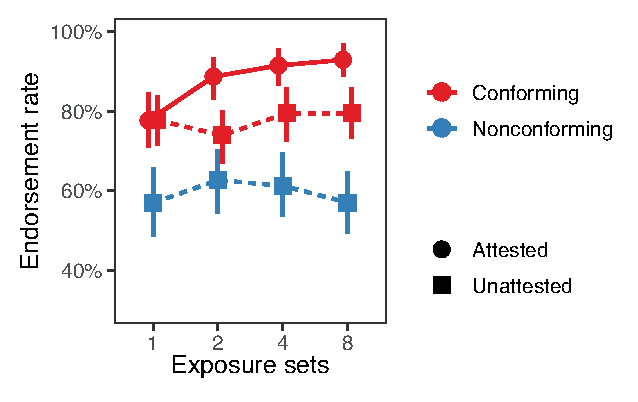
\includegraphics[scale=0.85]{../analysis/figures/LnG-results.eps}
\caption{Mean endorsement rates from Experiment 1 of \textcite{linzen2017rapid}. Error bars represent bootstrapped 95\% confidence intervals.}
\label{fig:lng}
\end{figure}

\section{Replication}

\subsection{Materials, procedure, \& participants}

All experimental materials used by \textcite{linzen2017rapid} were readily available on a GitHub repository.\footnote{\url{https://github.com/TalLinzen/rapid_phonotactic_generalization}}
Thus, the exact same audio stimuli were retrieved for use in the replication experiment.
However, as the web experiment framework ExperiGen used in the original experiment was no longer easily deployable, the experiment was adapted into a static site for use with the Stanford ALPS Lab experiment template.\footnote{\url{https://fauxneticien.github.io/phon-learning/experiment/?l1e4}, with the parameters \texttt{l1} for List 1 and \texttt{e4} for 4 exposure sets.}
While the presentation framework was different, substantive elements of the original experiment were retained (e.g. original JavaScript code for stimulus sampling, original question at test trials: ``Does this sound like it could be a word of the language you were listening to?'').
All materials used in the replication experiment are also readily available in a GitHub repository,\footnote{\url{https://github.com/fauxneticien/phon-learning}} and the experiment was also pre-registered.\footnote{\url{https://osf.io/jkm2a}}

Given the resource and time constraints of a class project, and to recuit additional participants per exposure condition, only the 1-set and 4-set exposure conditions were included in the replication experiment (though 109 participants were recruited for each condition, compared to the original 72 per condition).
Participants in the 1-set condition were paid \$0.50 and those in the 4-set condition were paid \$0.75 (calculated from a \$15/hour minimum wage and the expected duration of the experiment).

218 participants were recruited from MTurk (129 male, 88 female, 1 other; median age: 35, age range: 18-18, 1 unreported).
5 participants were removed as their reported native language was not English.
Thus, the analysis was conducted on data based on 213 participants.

\subsection{Analysis}

A Bayesian mixed-effects logistic regression was fitted to the data using the \texttt{brm} function from the \texttt{brms} R package \parencite{burkner2017brms}.
Endorsement (0 = does not belong to the language or 1 = belongs to the language) was modelled was a function of number of exposures (1- or 4-set of words; reference level 1), and onset type (conforming-attested, conforming-unattested, or nonconforming-unattested; reference level conforming-attested), and their two-way interaction.
The model included the maximal random-effect structure justified by the design: a by-subject intercept and slope for the effect of onset type, and by-onset intercepts and slopes for both onset type and number of exposures.
Default priors from the \texttt{brms} package were used.\footnote{I opted to use the default priors since I wasn't sure whether or how to specify explicit priors based on results from \textcite{linzen2017rapid}.}

Four sampling chains ran for 4000 iterations with a warm-up period of 2000 iterations for each model, yielding 8000 samples for each parameter tuple. 
For all relevant cell means and differences between them, the expected values under the posterior distribution and their 95\% credible intervals (CIs) are reported.
For differences between cells, the posterior probability that a difference δ is not equal to zero is reported.
Non-linear hypothesis testing was conducted using the \texttt{hypothesis} function from the \texttt{brms} package.

\section{Results}

The mean proportions of test words judged as acceptable by each exposure group for each of the stimulus types are shown in Figure \ref{fig:end}, with the left-panel for mean endorsement rates from \textcite{linzen2017rapid} for reference, and the right-panel for results from this replication experiment.

\begin{figure}[h]
\center
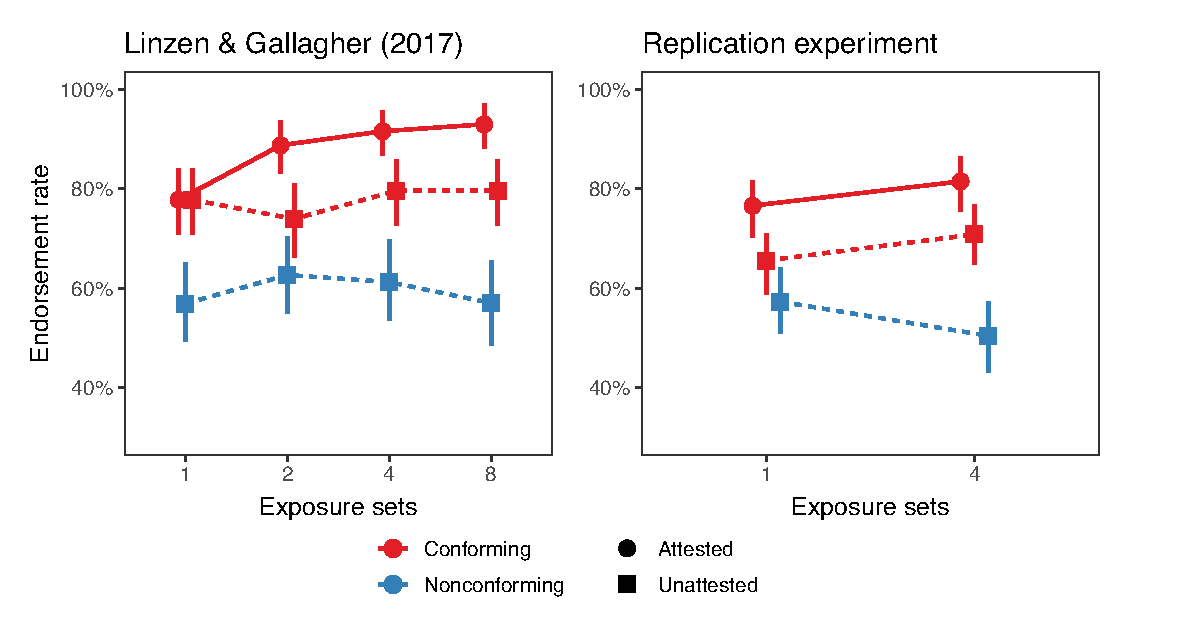
\includegraphics[scale=0.75]{../analysis/figures/endorsements.eps}
\caption{Mean endorsement rates from Experiment 1 of \textcite{linzen2017rapid} (left panel) and current replication experiment (right panel). Error bars represent bootstrapped 95\% confidence intervals.}
\label{fig:end}
\end{figure}

Results from the Bayesian mixed-effects logistic regression indicated that subjects in the 4-exposure condition were not more likely to endorse test words than those in the 1-exposure condition ($\beta = 0.33$, CI = [-0.24, 0.93], $P(\delta > 0) = .867$).
In the 1-exposure condition, subjects were less likely to endorse nonconforming and unattested test words than conforming and attested ones ($\beta = -0.95$, CI = [-1.48, -0.39], $P(\delta < 0) = .999$), but did not endorse conforming and unattested test words differently from conforming and attested ones ($\beta = -0.44$, CI = [-1.01, 0.16], $P(\delta < 0) = .930$).
Likewise, in the 4-exposure condition, subjects were less likely to endorse nonconforming and unattested test words than conforming and attested ones ($\beta = -1.09$, CI = [-2.11, -0.09], $P(\delta < 0) = .970$), but did not endorse conforming and unattested test words differently from conforming and attested ones ($\beta = -0.37$, CI = [-1.38, 0.62], $P(\delta < 0) = .730$).
Finally, while in the 4-exposure condition, subjects were less likely to endorse nonconforming and unattested test words than conforming and unattested ones ($\beta = -0.71$, CI = [-1.4, -0.05], $P(\delta < 0) = .960$), they did not endorse nonconforming and unattested test words differently to conforming and unattested ones in the 1-exposure condition ($\beta = -0.51$, CI = [-1.04, 0.02], $P(\delta < 0) = .940$).

\section{Discussion}

The original experiment by \textcite{linzen2017rapid} and this replication investigated how participants who listened to varying amounts of stimuli from an artificial language in an exposure stage then judged novel stimuli in a test stage that were identical, similar, or dissimilar to those previously heard.
The two key results from \textcite{linzen2017rapid} were that amount of exposure had no significant effect on mean endorsement rate and that, within all exposure conditions, nonconforming and unattested stimuli were endorsed significantly less than conforming and attested stimuli.
Both these results were replicated.

\textcite{linzen2017rapid} also found an interaction effect between amount of exposure and stimulus type.
While the presence of the interaction between these variables was replicated, the exact interactions were only partially replicated.
In both the original experiment and this replication, participants did not endorse conforming and unattested stimuli differently from conforming and attested ones, in neither the 1-set nor 4-set condition.
Similarly, in both experiments, participants endorsed nonconforming and unattested stimuli less frequently than conforming and unattested ones in the 4-set condition.
While \textcite{linzen2017rapid} found this same contrast in endorsement rates in the 1-set condition, participants in the 1-set condition of the replication experiment did not differ in their endorsement rates of nonconforming and unattested stimuli and conforming and unattested ones.

The partial replication with regards to the interaction between amount of exposure and stimulus type may be related to the highly similar nature of the stimuli, as discussed by \textcite[][p. 10]{linzen2017rapid}.
As noted by the authors, all exposure words had the same voicing and were of the CVCV shape with stress on the first syllable.
The apparent influence of these similarities seem to be reflected in both the original and replication experiments, where even the nonconforming and unattested stimuli were endorsed relatively highly (around 60\%).
\textcite[][p. 10]{linzen2017rapid} noted that ``test words that differed from the exposure words in more dimensions, such as \emph{ulpiuzi} or \emph{eh} would have been endorsed at a lower rate''.
While this experiment could not have added such stimuli, one future direction would be to further investigate additional differences in stimuli and their consequence to endorsement rates in the same limited exposure setting (recall participants in the 1-set listening to only one set of 5 words).

The results of the replication are compatible with the general argumentation of \textcite[][]{linzen2017rapid}.
That learners consistently endorse dissimilar sounds relatively less frequently than identical sounds after as few as 5 words is incompatible with models of phonotactic learning that posit a minimal exposure requirement.
That learners don't appear to differentiate identical sounds from similar ones is incompatible with models that do not posit a minimal exposure requirement but do posit that learners would readily differentiate between such sounds.
In this way, this replication experiment contributes additional empirical data to be reconciled by more adequate models which make explicit predictions about the time course of phonotactic learning and its relation to amount of exposure.

% On the other hand, there was only a partial replication with regards to stimulus type and the interaction between stimulus type and amount of exposure.
% The results that replicated were that a) nonconforming and unattested test words were less likely to be endorsed than conforming and attested ones in all exposure conditions and that b), in the 1-exposure condition, conforming and unattested test words were not endorsed differently from conforming and attested ones.
% Similarly, in the 4-exposure condition, conforming and unattested test words were not endorsed differently from conforming and attested ones, and this result does not replicate that from \textcite{linzen2017rapid}, who did find that 


% By contrast, \textcite{linzen2017rapid} found that conforming and unattested test words were 


% not endorsed differently from conforming and attested ones


\nocite{linzen2017rapid,san2020replication}
\printbibliography

\begin{filecontents}{report.bib}

@article{burkner2017brms,
    Author = {Bürkner, Paul-Christian},
    Date-Added = {2020-06-11 12:59:44 -0700},
    Date-Modified = {2020-06-11 13:03:55 -0700},
    Doi = {10.18637/jss.v080.i01},
    Journal = {Journal of Statistical Software},
    Number = {1},
    Pages = {1--28},
    Title = {{b}rms: An {R} package for {B}ayesian multilevel models using {S}tan},
    Volume = {80},
    Year = {2017}}

@article{linzen2017rapid,
    Author = {Linzen, Tal and Gallagher, Gillian},
    Date-Added = {2020-06-06 12:38:45 -0700},
    Date-Modified = {2020-06-11 13:03:22 -0700},
    Doi = {10.5334/labphon.44},
    Journal = {Laboratory Phonology: Journal of the Association for Laboratory Phonology},
    Number = {1},
    Publisher = {Ubiquity Press},
    Title = {Rapid generalization in phonotactic learning},
    Volume = {8},
    Year = {2017}}

\end{filecontents}

\end{document}